\documentclass[11pt,a4paper]{article}
\usepackage[utf8]{inputenc}
\usepackage[T1]{fontenc}
\usepackage[french]{babel}
\usepackage{graphicx}
\usepackage{booktabs}
\usepackage{geometry}
\usepackage{hyperref}
\geometry{margin=2.5cm}

\title{Clustering des données immobilières californiennes}
\author{Bloc IA --- Prosit 1}
\date{25 mars 2026}

\begin{document}
\maketitle

\section{Description des données}

Le jeu de données \texttt{housing.csv} contient 20\,640 enregistrements issus du recensement californien de 1990. Chaque ligne correspond à un \textit{block group} (plus petite unité administrative, 500 à 5\,000 habitants).

\begin{table}[h]
\centering
\caption{Variables du dataset}
\begin{tabular}{lll}
\toprule
Variable & Type & Description \\
\midrule
longitude / latitude & float & Coordonnées géographiques \\
housing\_median\_age & float & Âge médian des logements \\
total\_rooms & float & Nombre total de pièces \\
total\_bedrooms & float & Nombre total de chambres \\
population & float & Population du block group \\
households & float & Nombre de ménages \\
median\_income & float & Revenu médian (en dizaines de k\$) \\
median\_house\_value & float & Prix médian du logement (\$) \\
ocean\_proximity & cat. & Proximité à l'océan \\
\bottomrule
\end{tabular}
\end{table}

Valeurs manquantes : seule \texttt{total\_bedrooms} présentait 207 valeurs nulles. Ces valeurs ont été imputées à l'aide de \textbf{KNNImputer} (k=5, pondération par distance) en utilisant l'ensemble des autres variables numériques. Le dataset imputé est exporté dans \texttt{data/housing\_data\_knn.csv}.

\section{Choix méthodologiques}

\begin{enumerate}
    \item \textbf{Imputation des valeurs manquantes} : KNNImputer (k=5, \texttt{weights='distance'}) après standardisation. Chaque valeur manquante de \texttt{total\_bedrooms} est prédite à partir de ses 5 plus proches voisins complets.
    \item \textbf{Variables} : toutes les colonnes du dataset sont utilisées. \texttt{ocean\_proximity} est encodée via \texttt{LabelEncoder} pour la rendre numérique.
    \item \textbf{Pas de standardisation} : les données brutes sont utilisées directement pour le clustering.
    \item \textbf{Algorithme} : KMeans --- simple, rapide et bien adapté aux données numériques continues. Paramètres : \texttt{n\_init=10}, \texttt{random\_state=42}.
    \item \textbf{Choix de k} : déterminé par \textbf{CAH} (Classification Ascendante Hiérarchique, méthode de Ward) via un dendrogramme (figure~\ref{fig:dendro}), puis validé par la méthode du coude (Elbow Method) sur le WCSS (figure~\ref{fig:elbow}). Les deux approches convergent vers $k = 5$.
\end{enumerate}

\begin{figure}[h]
\centering
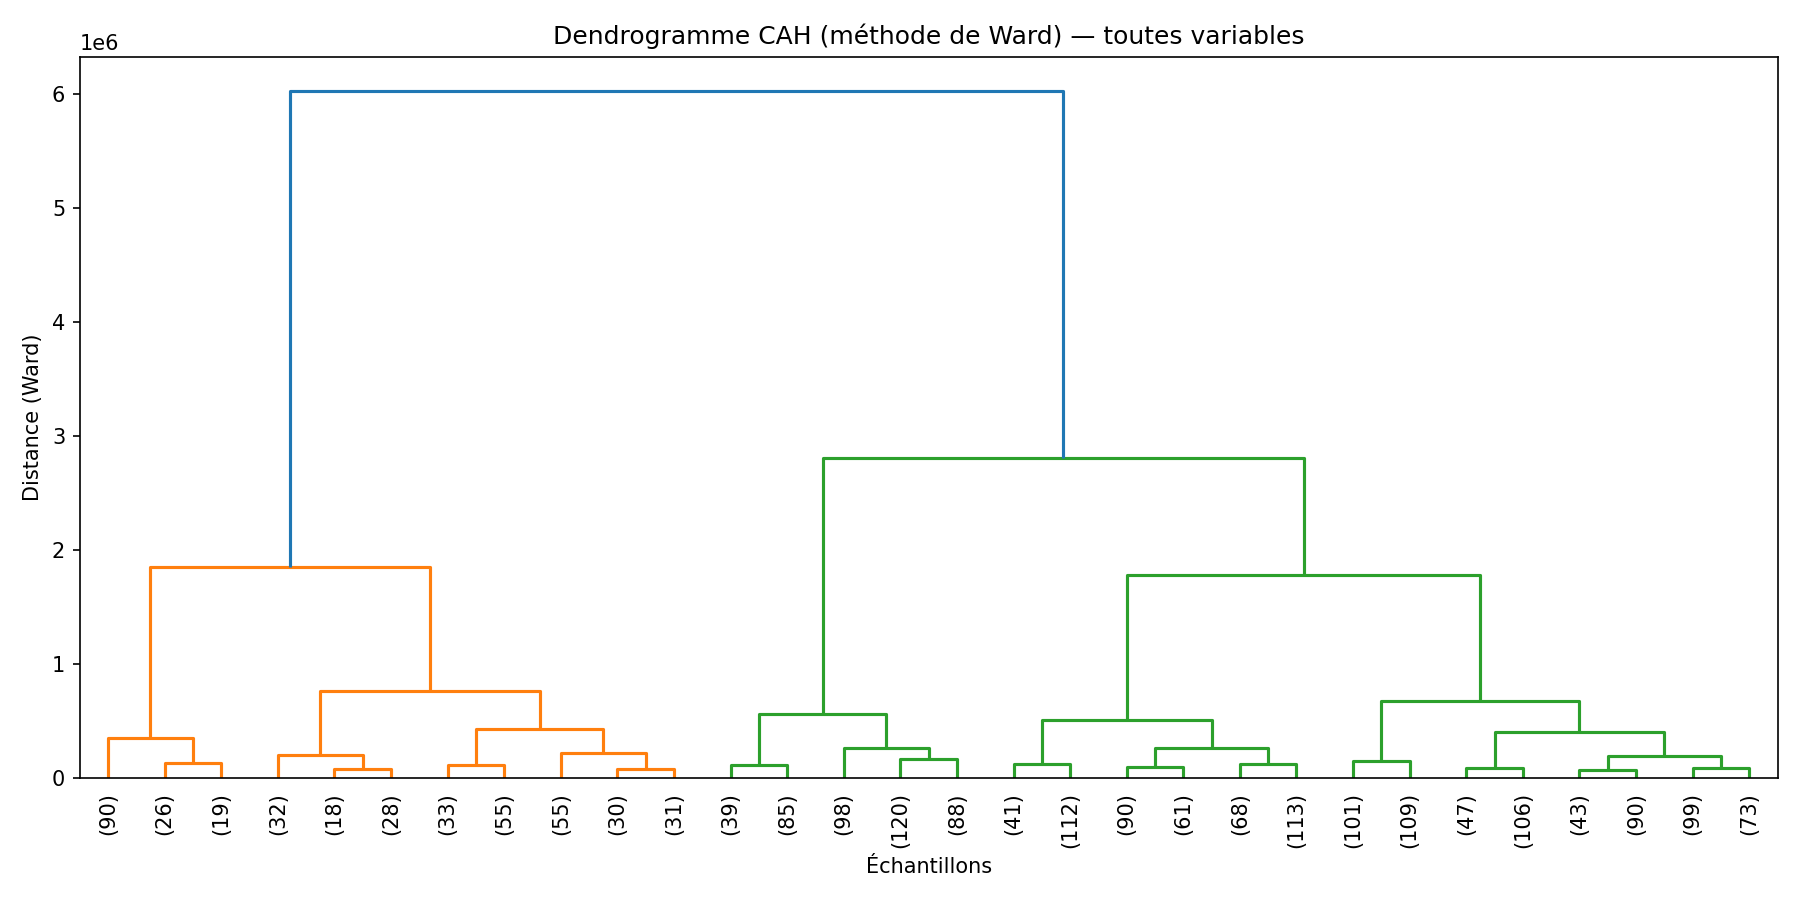
\includegraphics[width=0.85\textwidth]{data/dendrogram_cah.png}
\caption{Dendrogramme CAH (méthode de Ward) --- échantillon de 2\,000 points}
\label{fig:dendro}
\end{figure}

\begin{figure}[h]
\centering
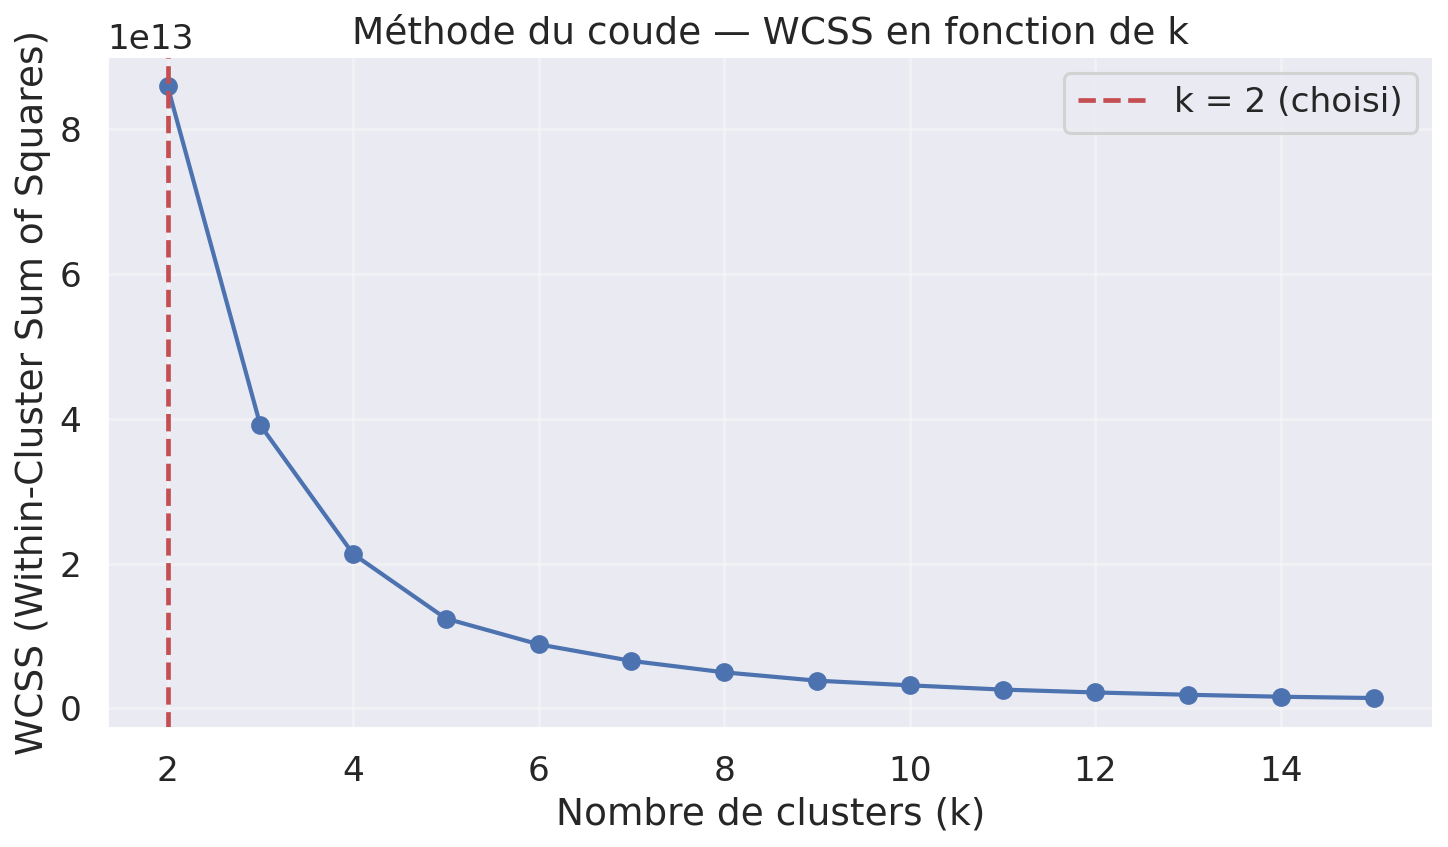
\includegraphics[width=0.85\textwidth]{data/elbow_method.png}
\caption{Méthode du coude --- WCSS en fonction de k}
\label{fig:elbow}
\end{figure}

\section{Résultats}

\subsection{Distribution des clusters}

\begin{table}[h]
\centering
\caption{Statistiques par cluster (k = 5)}
\begin{tabular}{crrr}
\toprule
Cluster & Effectif & Prix moyen (\$) & Revenu moyen \\
\midrule
0 & 5\,731 & 90\,084 & 2.50 \\
1 & 2\,318 & 346\,896 & 5.24 \\
2 & 6\,446 & 164\,722 & 3.47 \\
3 & 1\,613 & 480\,484 & 7.02 \\
4 & 4\,532 & 245\,435 & 4.35 \\
\bottomrule
\end{tabular}
\end{table}

\subsection{Visualisation géographique}

\begin{figure}[h]
\centering
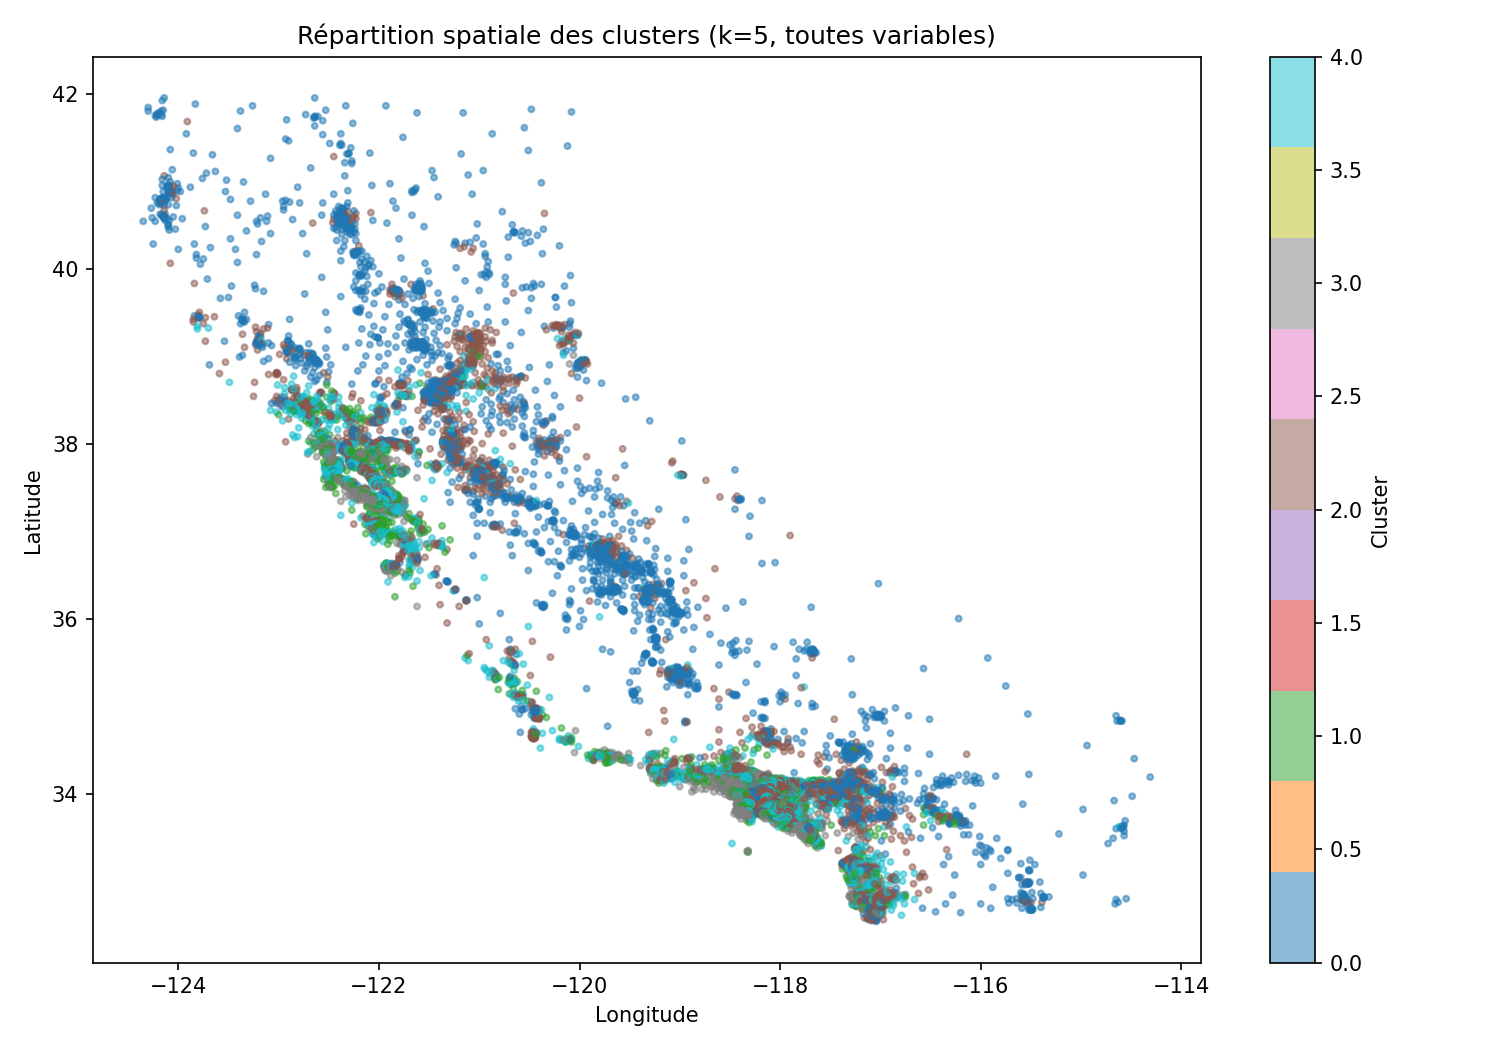
\includegraphics[width=0.85\textwidth]{data/clusters_scatter.png}
\caption{Répartition spatiale des clusters (latitude vs longitude)}
\end{figure}

\subsection{Interprétation synthétique}

\begin{itemize}
    \item Le clustering segmente la Californie en 5 profils socio-économiques distincts.
    \item Le \textbf{cluster 0} (5\,731 block groups) regroupe les zones les moins chères avec les revenus les plus bas --- zones rurales et intérieures.
    \item Le \textbf{cluster 3} (1\,613 block groups) isole les zones les plus chères avec les revenus les plus élevés (prix moyen 480\,484\,\$, revenu 7.02).
    \item Les \textbf{clusters 1, 2, 4} représentent des profils intermédiaires à différents niveaux de prix et de revenus.
    \item Le dataset final, enrichi de la colonne \texttt{cluster}, est exporté dans \texttt{data/housing\_data\_knn\_clustered.csv}.
\end{itemize}

\section{Analyse exploratoire et interprétation}

\subsection{Qualité des données --- valeurs plafonnées}

Deux variables présentent un \textbf{plafonnement artificiel} visible dans leurs distributions (figure~\ref{fig:capped}) :

\begin{itemize}
    \item \texttt{median\_house\_value} est plafonné à 500\,001\,\$ pour \textbf{965 block groups} (4.7\,\%). Ces zones, probablement les plus chères (Beverly Hills, Palo Alto\ldots), ont leur prix réel tronqué. Cela biaise toute analyse des hauts de gamme et peut fausser le clustering en regroupant artificiellement des zones de prix très différents.
    \item \texttt{housing\_median\_age} est plafonné à 52 ans pour \textbf{1\,273 block groups} (6.2\,\%). Les bâtiments les plus anciens sont donc indistinguables dans le dataset.
\end{itemize}

\begin{figure}[h]
\centering
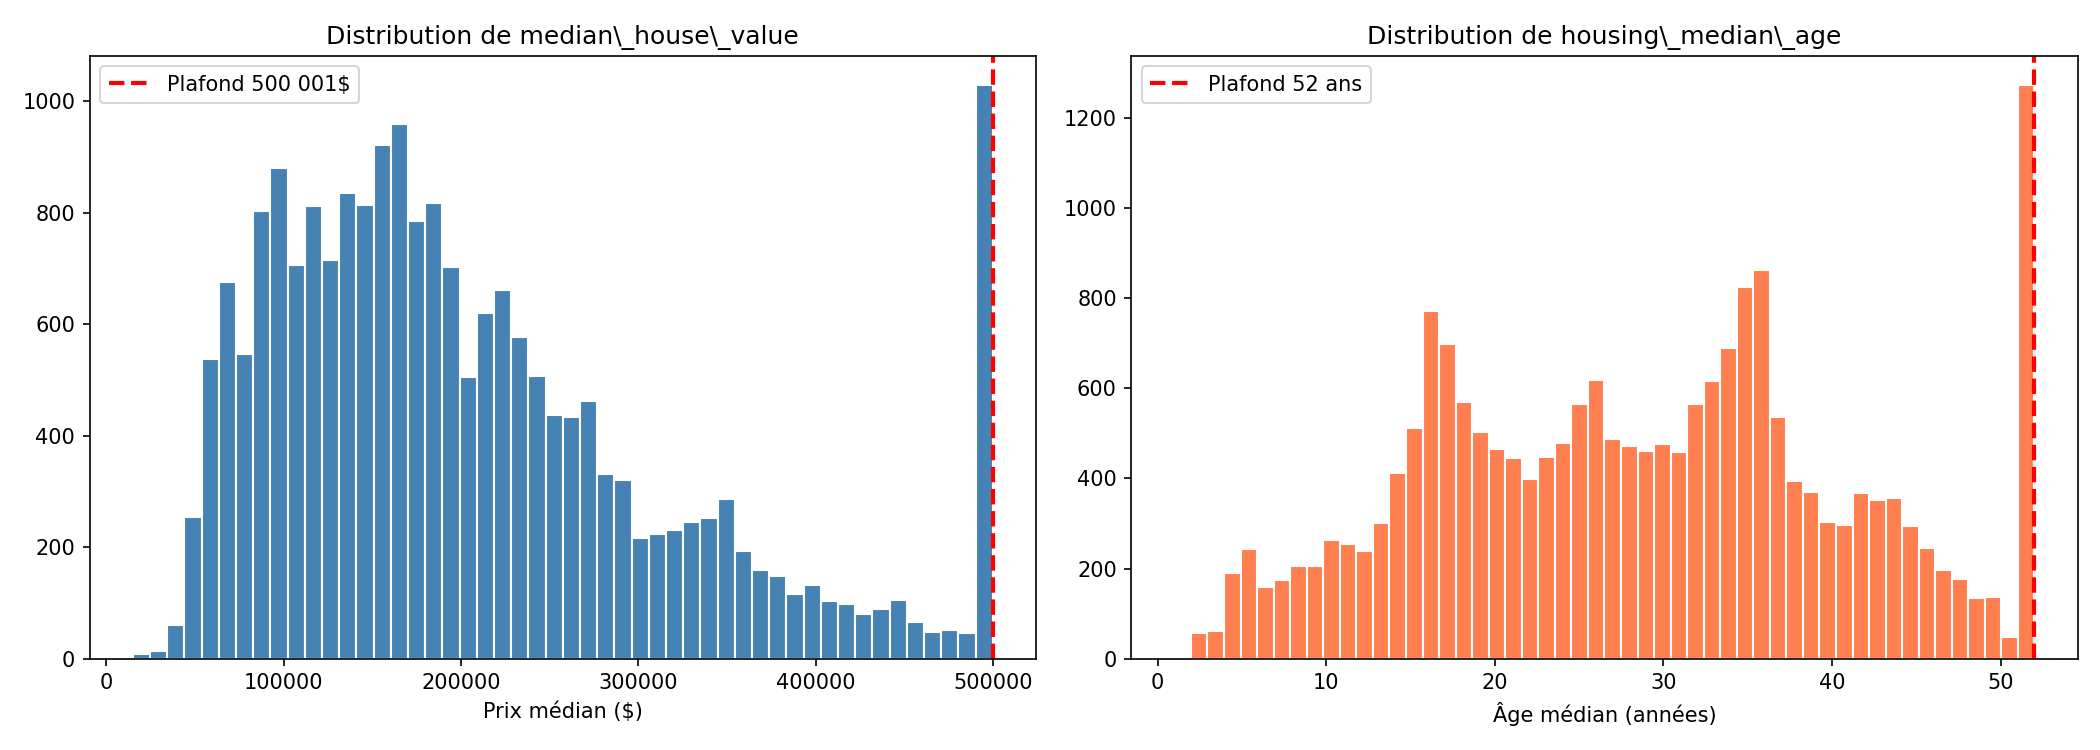
\includegraphics[width=0.95\textwidth]{data/capped_values.png}
\caption{Distributions avec valeurs plafonnées (pics visibles aux bornes)}
\label{fig:capped}
\end{figure}

\subsection{Revenu et prix --- la corrélation dominante}

Le revenu médian est de loin le meilleur prédicteur du prix ($r = 0.69$), bien devant toutes les autres variables. La figure~\ref{fig:income} montre cette relation quasi-linéaire, avec deux anomalies notables :

\begin{itemize}
    \item Une \textbf{ligne horizontale à 500\,001\,\$} : les valeurs plafonnées, qui créent un artefact visuel et statistique.
    \item Des \textbf{zones à haut revenu mais prix modéré} (coin bas-droit) : possiblement des zones rurales aisées avec un foncier bon marché.
\end{itemize}

\begin{figure}[h]
\centering
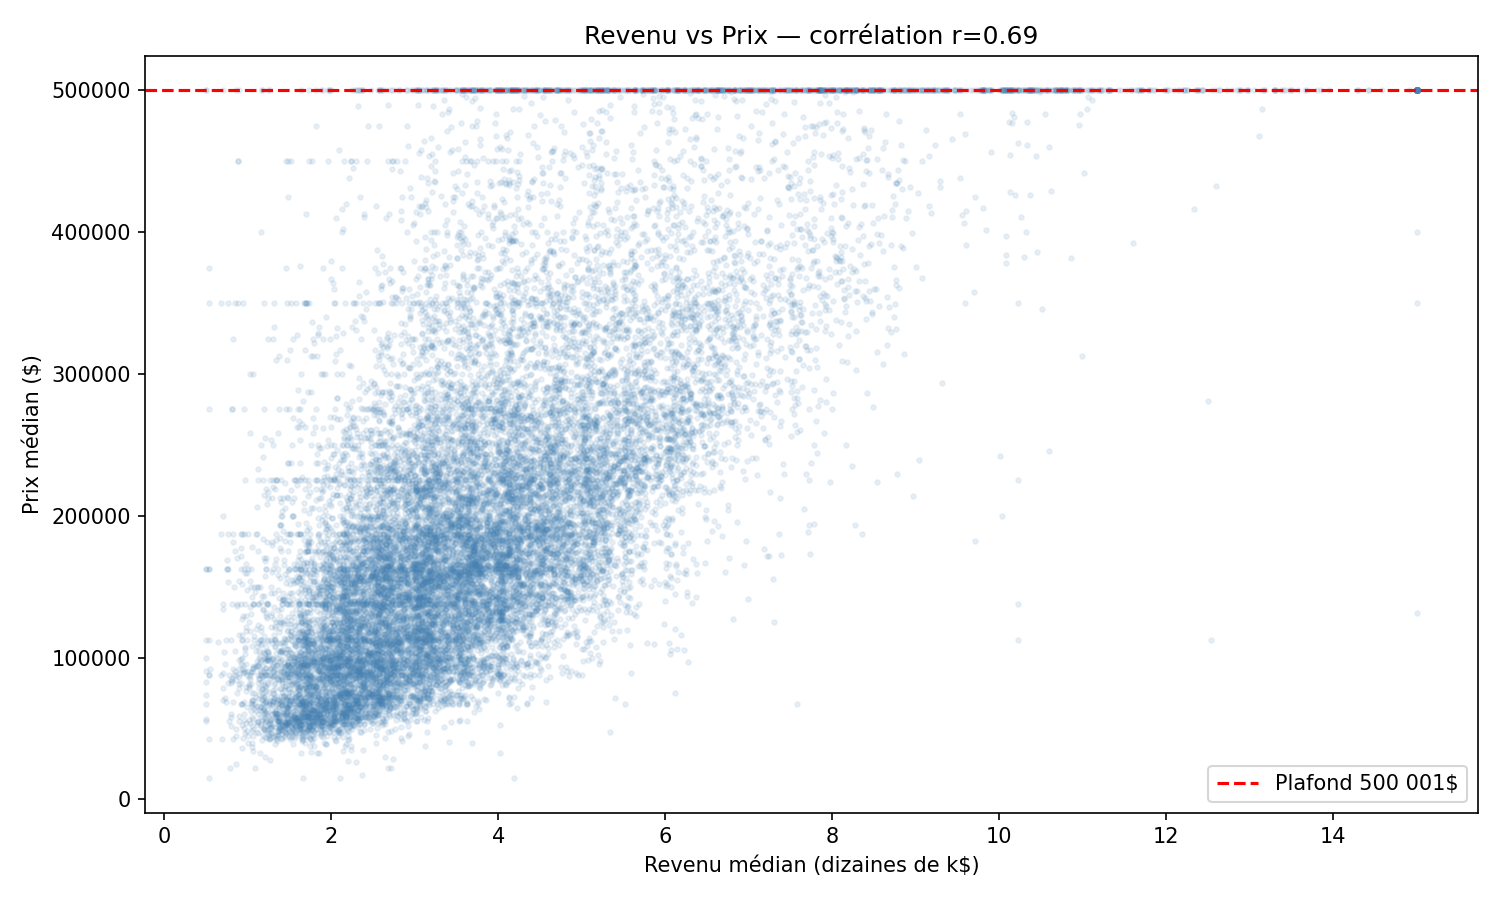
\includegraphics[width=0.85\textwidth]{data/income_vs_price.png}
\caption{Revenu médian vs prix --- corrélation $r = 0.69$}
\label{fig:income}
\end{figure}

\subsection{L'effet côtier}

La proximité à l'océan a un impact majeur sur les prix (figure~\ref{fig:ocean}). Les zones \texttt{INLAND} affichent un prix médian de 108\,500\,\$, contre 233\,800\,\$ pour \texttt{NEAR BAY} --- plus du double. La catégorie \texttt{ISLAND} (5 observations seulement) montre des prix très élevés mais n'est pas statistiquement significative.

\begin{figure}[h]
\centering
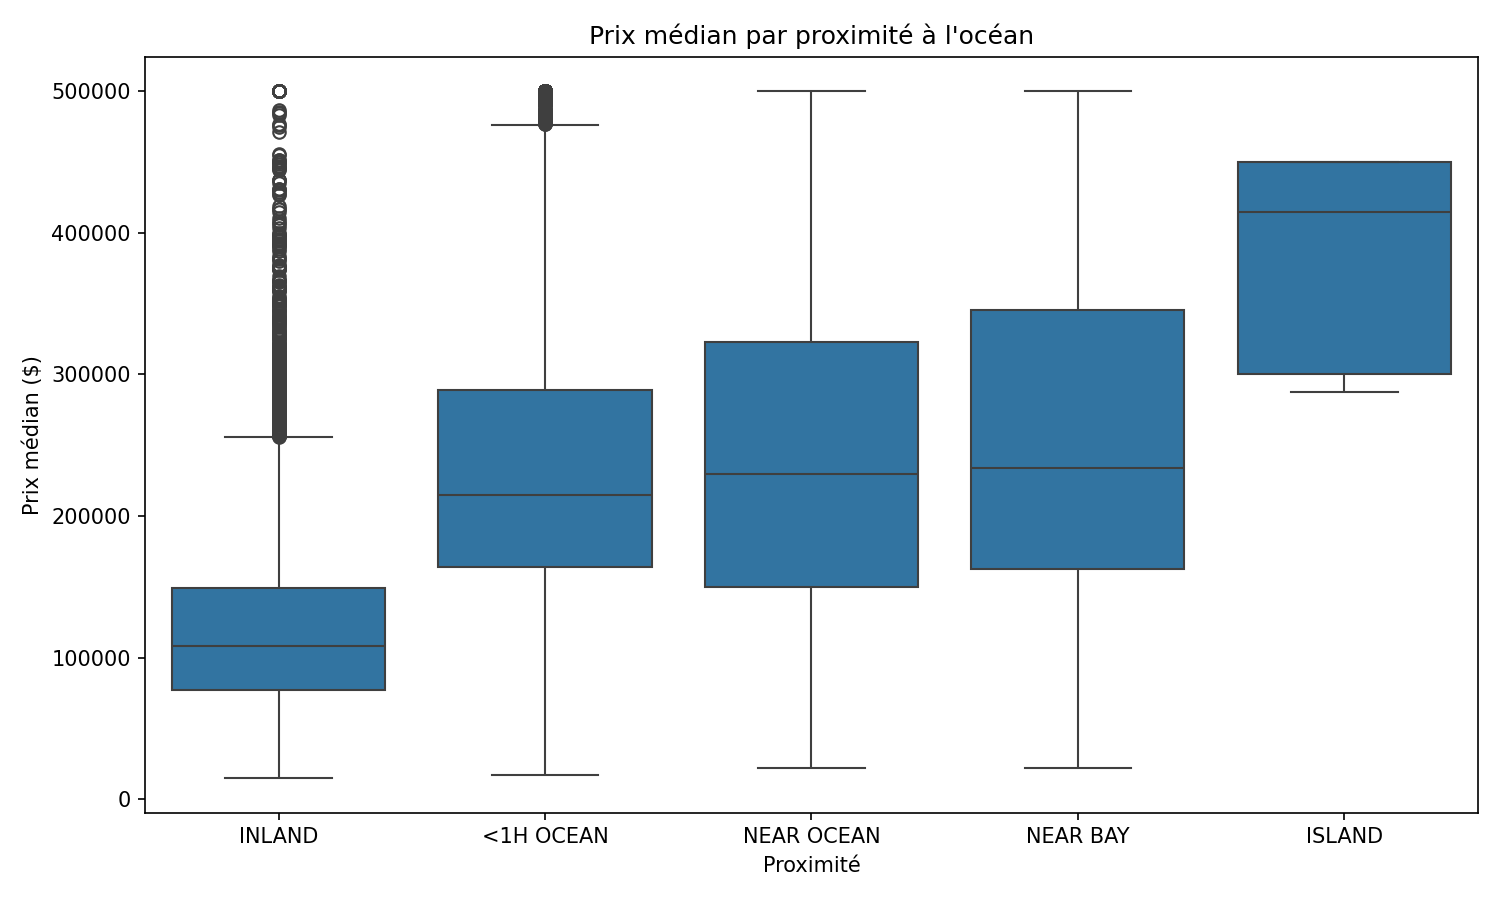
\includegraphics[width=0.85\textwidth]{data/price_by_ocean.png}
\caption{Prix médian par proximité à l'océan}
\label{fig:ocean}
\end{figure}

La majorité des block groups (44.3\,\%) se trouvent à moins d'une heure de l'océan, et près d'un tiers (31.7\,\%) sont situés en zone intérieure.

Ce déséquilibre explique en partie la structure du clustering. La Californie est un État profondément dual : une frange côtière densément peuplée et chère, et un vaste intérieur agricole et résidentiel à prix modéré. La variable \texttt{ocean\_proximity} est intégrée au clustering via un encodage \texttt{LabelEncoder}, ce qui permet au modèle de capter directement cette dimension côtière en complément des coordonnées géographiques.

\subsection{Matrice de corrélation}

La figure~\ref{fig:corr} révèle plusieurs structures intéressantes :

\begin{itemize}
    \item \texttt{total\_rooms}, \texttt{total\_bedrooms}, \texttt{population} et \texttt{households} sont fortement corrélés entre eux ($r > 0.85$). Ce sont des mesures de \textbf{taille du block group} : un quartier plus peuplé a logiquement plus de pièces, de chambres et de ménages. Utiliser ces 4 variables simultanément dans un modèle introduirait de la \textbf{multicolinéarité}.
    \item \texttt{latitude} et \texttt{longitude} captent la géographie : les prix baissent quand on s'éloigne de la côte (latitude élevée = nord, corrélation négative avec le prix).
    \item \texttt{median\_income} est la seule variable fortement corrélée au prix ($r = 0.69$) sans être redondante avec les autres.
\end{itemize}

\begin{figure}[h]
\centering
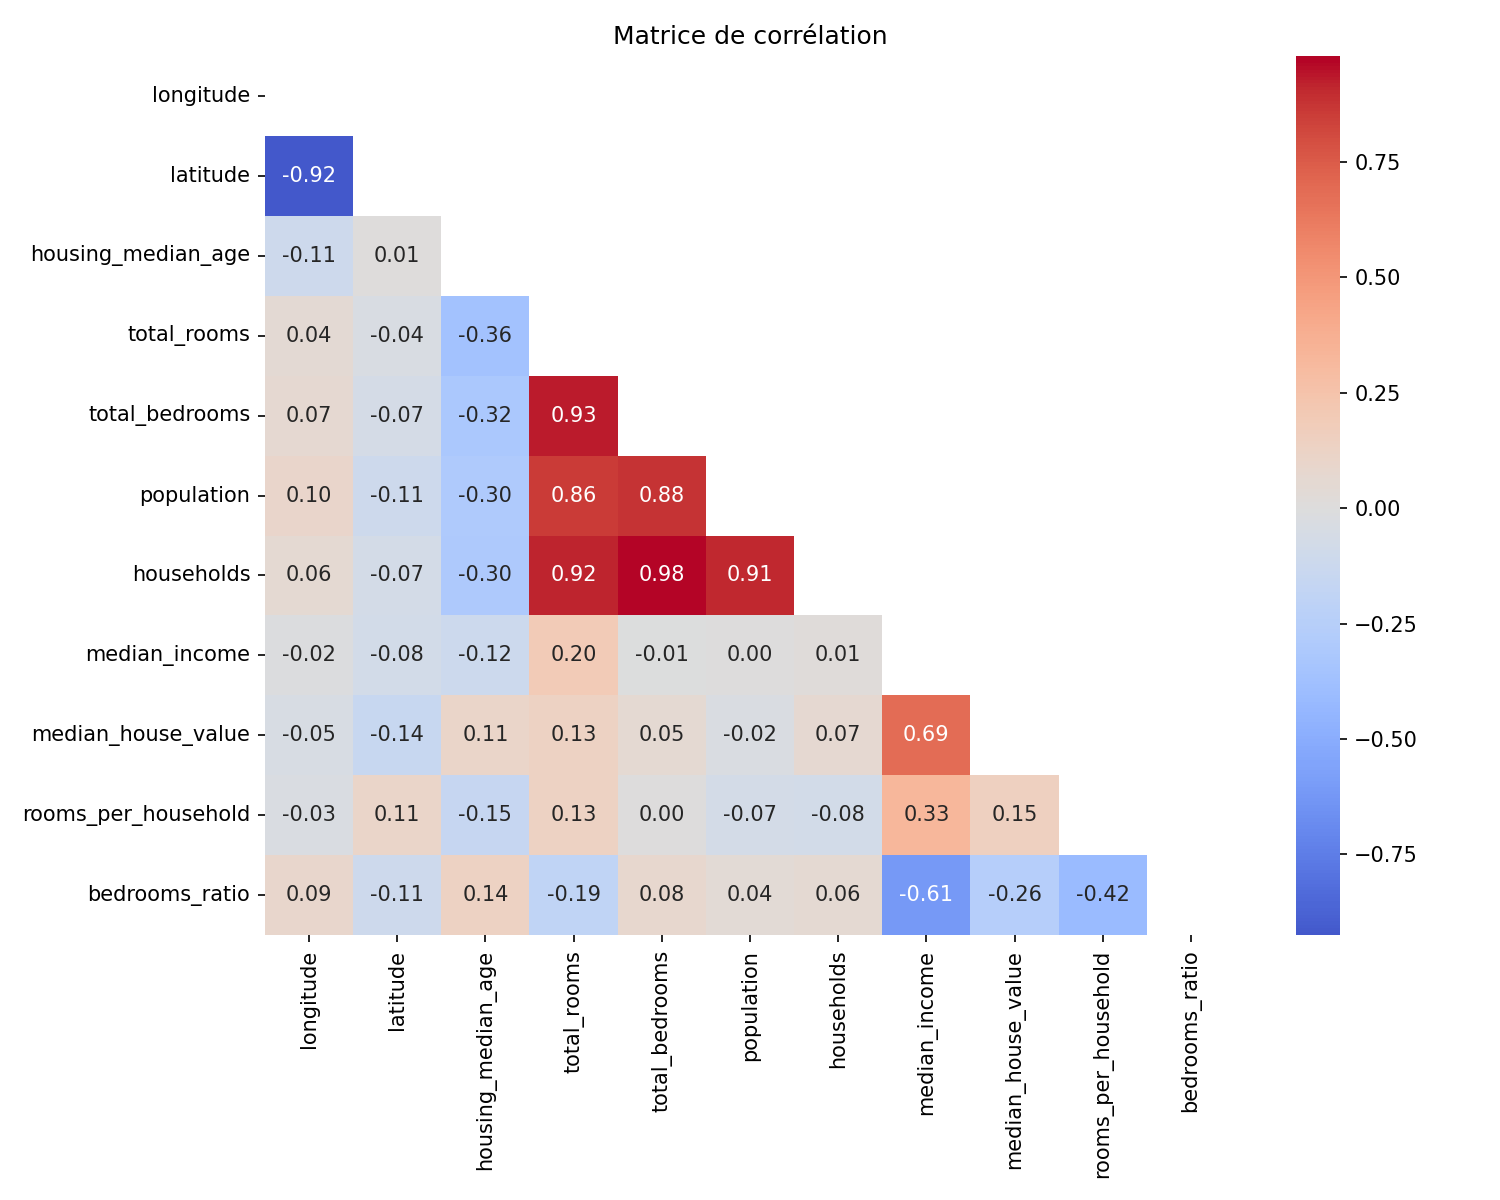
\includegraphics[width=0.85\textwidth]{data/correlation_heatmap.png}
\caption{Matrice de corrélation des variables numériques}
\label{fig:corr}
\end{figure}

Malgré la multicolinéarité entre les variables de taille, toutes les variables sont conservées dans le clustering. Sans standardisation, ce sont les variables à grande échelle (\texttt{median\_house\_value}, \texttt{total\_rooms}, \texttt{population}) qui dominent naturellement le calcul de distance euclidienne, ce qui oriente le clustering vers une segmentation principalement économique et démographique.

\subsection{Variables dérivées --- le ratio chambres/pièces}

En créant le ratio \texttt{bedrooms\_ratio} = \texttt{total\_bedrooms} / \texttt{total\_rooms}, on obtient une corrélation négative avec le prix ($r = -0.26$). Les logements avec une \textbf{proportion élevée de chambres} par rapport au nombre total de pièces sont moins chers. Cela correspond à des logements plus petits (studios, T1) où la chambre constitue l'essentiel de l'espace, typiques des zones à faible revenu.

\begin{figure}[h]
\centering
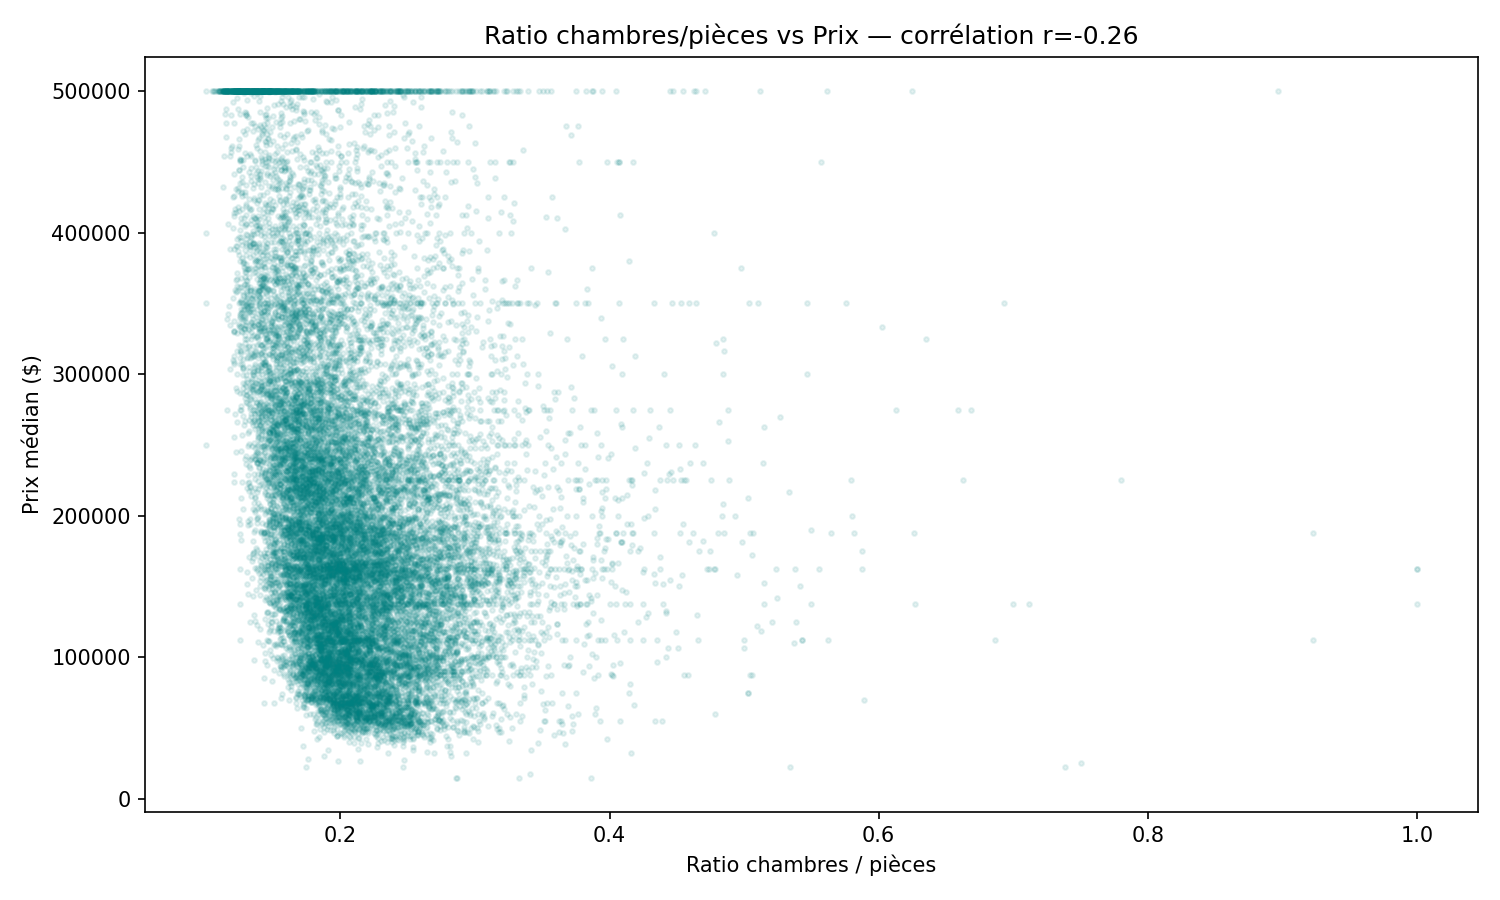
\includegraphics[width=0.85\textwidth]{data/bedrooms_ratio_vs_price.png}
\caption{Ratio chambres/pièces vs prix --- corrélation $r = -0.26$}
\label{fig:bedrooms}
\end{figure}

À l'inverse, un ratio faible signale des logements spacieux avec salon, bureau, salle à manger --- typiques des quartiers résidentiels aisés. Cette variable dérivée est plus informative que \texttt{total\_bedrooms} seul ($r = 0.05$ avec le prix) car elle normalise par la taille du logement et capture réellement la \textbf{structure} du bien plutôt que sa taille brute. Dans un modèle prédictif, ce ratio serait un candidat pertinent en remplacement des variables brutes \texttt{total\_rooms} et \texttt{total\_bedrooms}.

\subsection{Outliers et données suspectes}

Quelques observations extrêmes méritent attention :

\begin{itemize}
    \item \textbf{33 block groups} ont plus de 20\,000 pièces totales, et \textbf{9} ont plus de 50 pièces par ménage. Ces valeurs sont physiquement improbables et pourraient résulter d'erreurs de saisie ou de block groups atypiques (résidences universitaires, casernes).
    \item \textbf{23 block groups} dépassent 10\,000 habitants, avec un maximum à 35\,682 --- inhabituellement élevé pour la plus petite division administrative.
    \item Le ratio \texttt{population\_per\_household} atteint 1\,243 pour un block group, ce qui est manifestement une erreur (moyenne = 3.07).
\end{itemize}

Ces anomalies n'ont pas été filtrées dans le pipeline actuel mais devraient l'être dans un contexte de modélisation prédictive.

\section{Évaluation du clustering --- Analyse Silhouette}

Le score silhouette mesure pour chaque point la qualité de son assignation : $s = (b - a) / \max(a, b)$, où $a$ est la distance moyenne aux points de son propre cluster et $b$ la distance moyenne aux points du cluster le plus proche. Un score de +1 indique un point parfaitement classé, 0 un point à la frontière, et un score négatif un point probablement mal assigné.

\subsection{Score silhouette en fonction de k}

La figure~\ref{fig:silscores} montre l'évolution du score silhouette moyen pour $k \in [2, 10]$. Le choix de $k = 5$ offre un compromis entre granularité de la segmentation et qualité du clustering.

\begin{figure}[h]
\centering
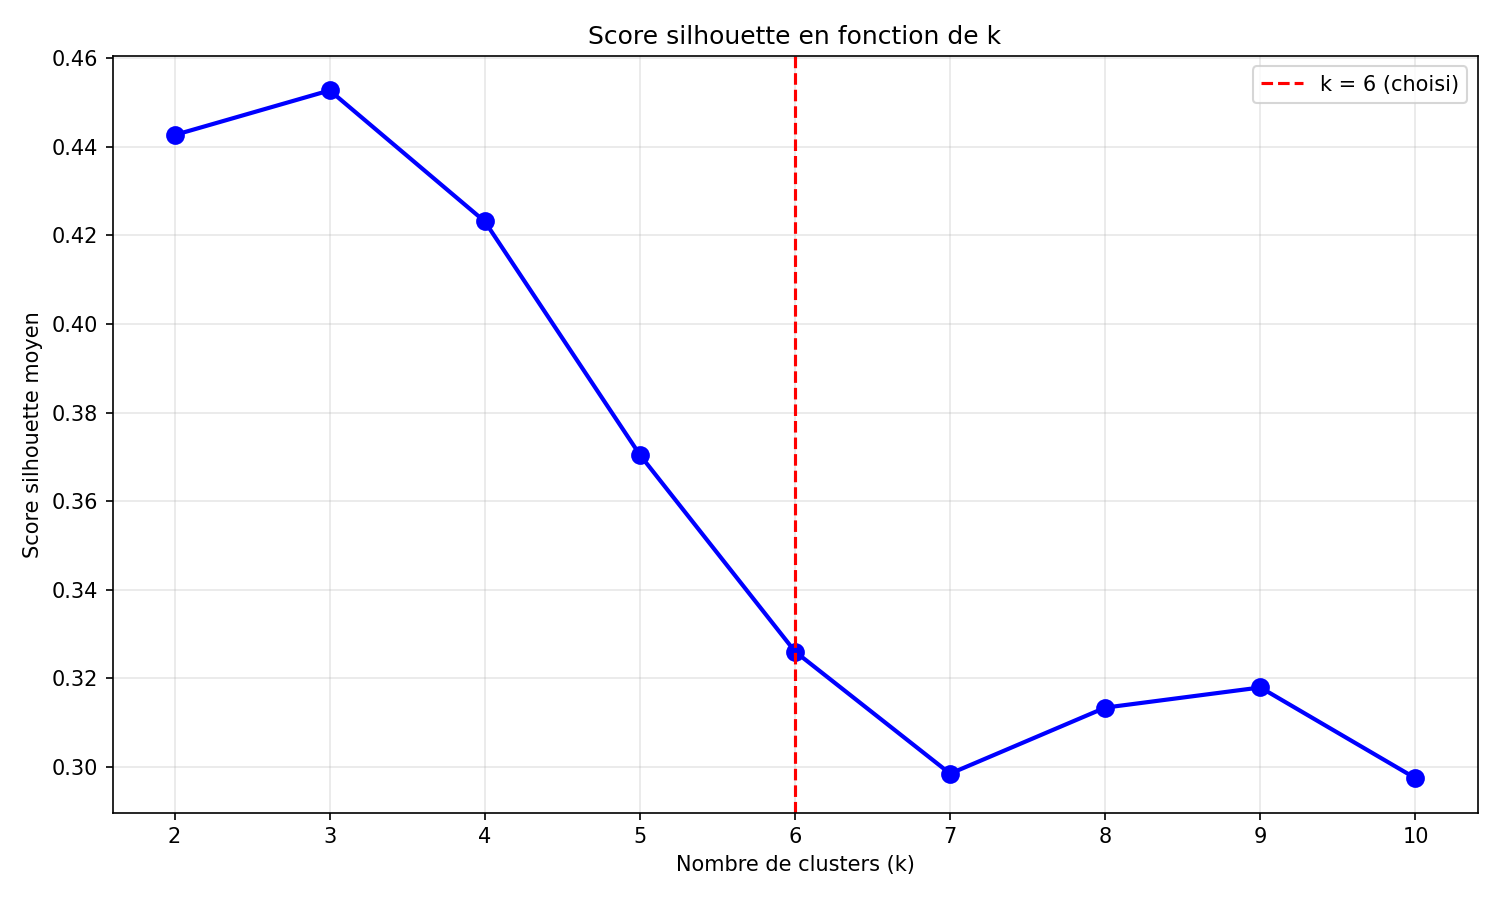
\includegraphics[width=0.85\textwidth]{data/silhouette_scores.png}
\caption{Score silhouette moyen en fonction de k}
\label{fig:silscores}
\end{figure}

\subsection{Silhouette plot détaillé (k=5)}

La figure~\ref{fig:silplot} détaille la distribution du score silhouette pour chaque cluster. L'analyse silhouette doit être re-exécutée avec les nouveaux paramètres ($k = 5$, toutes variables, sans standardisation) via le notebook \texttt{silhouette\_analysis.ipynb}.

\begin{figure}[h]
\centering
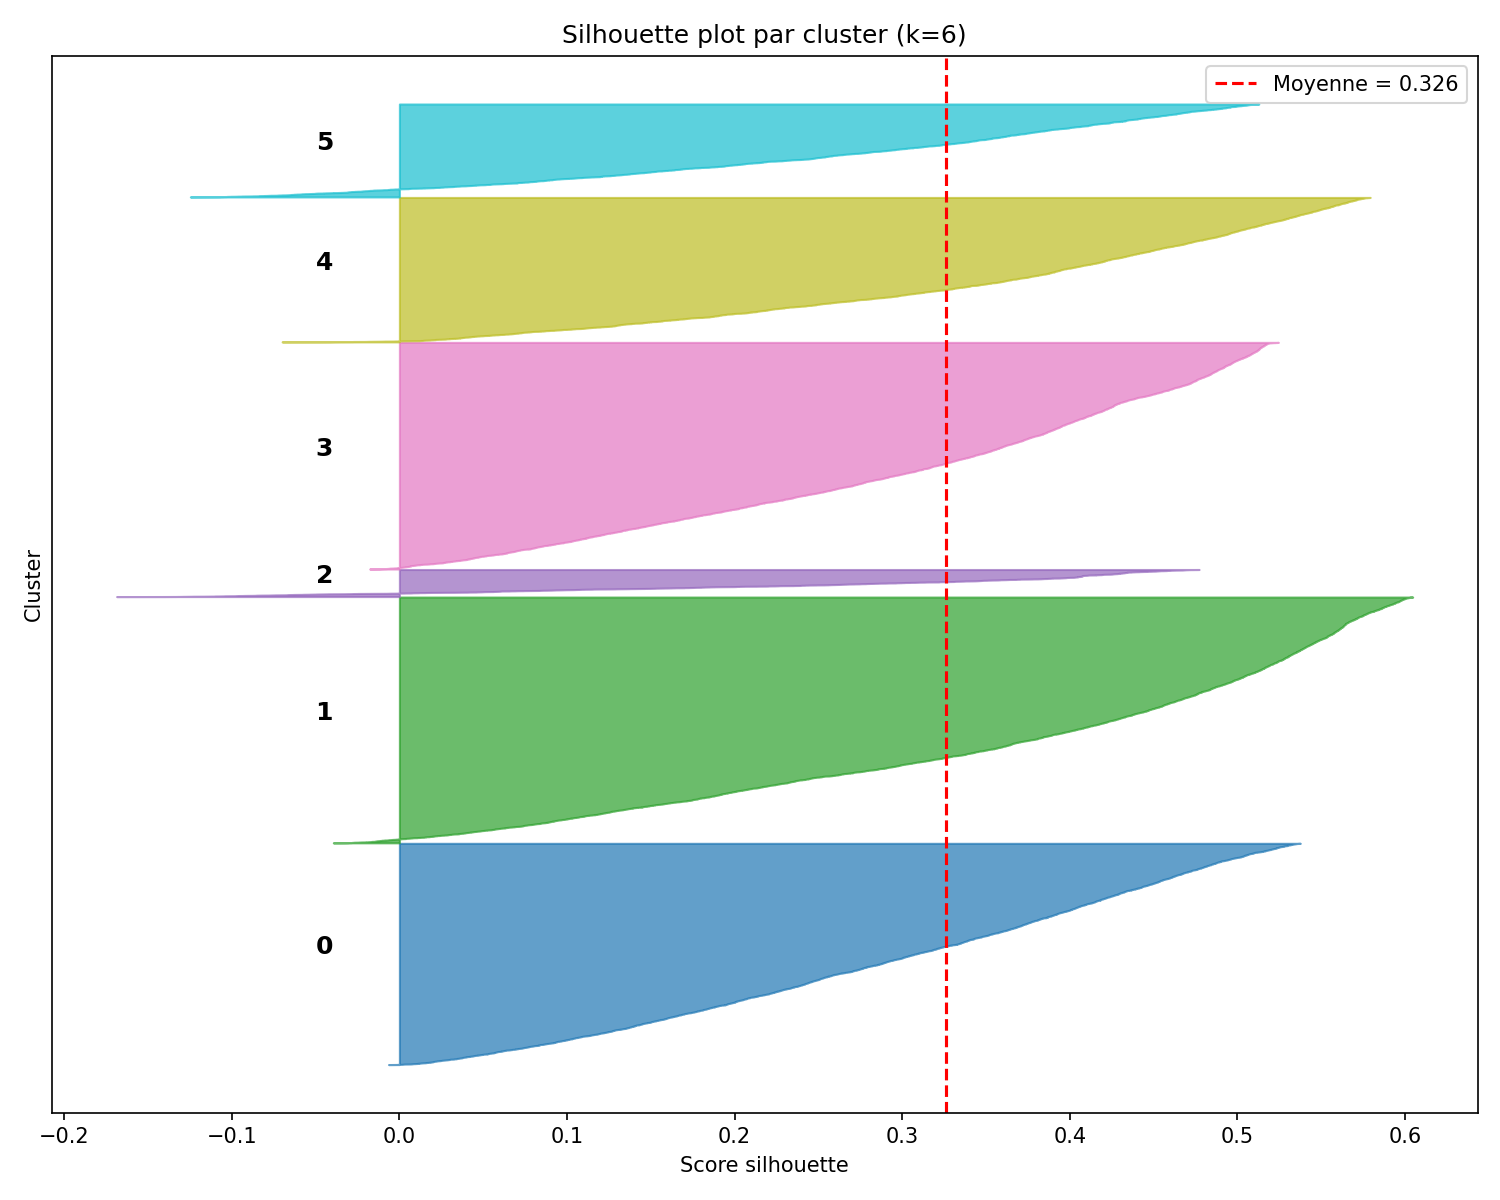
\includegraphics[width=0.85\textwidth]{data/silhouette_plot.png}
\caption{Silhouette plot par cluster (k=5)}
\label{fig:silplot}
\end{figure}

\subsection{Interprétation}

Le score silhouette permet d'identifier les clusters les plus cohérents (score élevé, peu de points négatifs) et les plus fragiles (score faible, proportion importante de points mal assignés). Les clusters à score négatif élevé indiquent des zones de transition entre segments, ce qui est attendu dans un espace géographique continu.

\section{Pipeline de transformation}

\begin{enumerate}
    \item Chargement de \texttt{housing.csv} (20\,640 lignes, 10 colonnes)
    \item Imputation de \texttt{total\_bedrooms} via KNNImputer (k=5) $\rightarrow$ \texttt{housing\_data\_knn.csv}
    \item Encodage de \texttt{ocean\_proximity} via \texttt{LabelEncoder}
    \item Détermination de $k$ par CAH (dendrogramme de Ward)
    \item Validation par méthode du coude (WCSS) $\rightarrow$ $k = 5$
    \item KMeans ($k = 5$) sur toutes les variables $\rightarrow$ ajout de la colonne \texttt{cluster}
    \item Export $\rightarrow$ \texttt{housing\_data\_knn\_clustered.csv} (20\,640 lignes, 11 colonnes)
\end{enumerate}

\section*{Dépôt GitHub}

Le code source complet (notebooks, données, rapport) est disponible à l'adresse :\\
\url{https://github.com/Anisse-Imer/bloc-ia-prosit-1-clustering}

\end{document}
